\chapter{Methodology}
\label{chap:methodology}

\section{Framework Overview}

KGE-NFM (Knowledge graph embedding - Neural Factorization Machine) is the main DTI prediction framework studied in this project. It uses
a two-stage design. First, a knowledge graph encoder learns drug and protein
representations from biomedical triples. Second, these representations are
combined with structural descriptors and processed by a Neural Factorization
Machine (NFM) to predict DTI labels.

This project evaluates two alternative encoder configurations within the same
framework: DistMult and CompGCN. The remaining stages, including feature
construction, preprocessing, NFM architecture, and evaluation data, are kept
consistent to support a controlled encoder comparison.

\begin{equation}
    \text{Biomedical KG}
    \rightarrow
    \left\{
        \begin{array}{c}
            \text{DistMult}\\
            \text{CompGCN}
        \end{array}
    \right.
    \rightarrow
    \text{drug/protein embeddings}
    \rightarrow
    \text{NFM}
    \rightarrow
    \text{DTI probability}.
\end{equation}

The first stage operates on a fold-specific biomedical knowledge graph. The
graph combines supporting biomedical relations with the positive DTI triples
available in the current training fold. This construction allows drug and
protein representations to reflect not only direct interaction evidence, but
also their connections to pathways, functions, domains, diseases, and other
biomedical entities. Test DTI labels are excluded from this graph so that the
learned representations do not contain information from the evaluation set.

DistMult and CompGCN provide two different mechanisms for constructing the KG
embeddings. DistMult learns entity representations through a diagonal
bilinear triple-scoring objective. CompGCN additionally enriches entity
representations through relation-aware neighborhood aggregation. These
encoders are treated as alternative configurations rather than sequential
components: a KGE-NFM experiment uses either DistMult embeddings or CompGCN
embeddings for a given run.

The output of the KGE stage is a separate embedding for the drug and protein
in each candidate pair. These embeddings represent relational biomedical
context, but they do not replace intrinsic entity information. The framework
therefore retains the Morgan fingerprint of the drug and the CTD descriptor
of the protein as two additional feature fields. Before prediction, all four
fields are scaled using parameters estimated from the training data, and the
KG embeddings may optionally be reduced using PCA.

In the second stage, NFM projects the heterogeneous fields into a common
latent space and applies Bi-Interaction pooling to model pairwise interactions
among them. Its neural prediction layers then produce the final DTI
probability. The KGE and NFM stages are trained sequentially rather than as a
single end-to-end network. Consequently, differences between the two model
configurations can be attributed primarily to the KG encoder while the
descriptor fields and downstream predictor remain unchanged. The complete
data flow is summarized in Figure~\ref{fig:kge_nfm_architecture}.

% Replace document/images/chapter5_overall_architecture.pdf with the final
% architecture diagram. The image is loaded automatically when it exists.
\begin{figure}[H]
\centering
\IfFileExists{images/chapter5_overall_architecture.pdf}{
    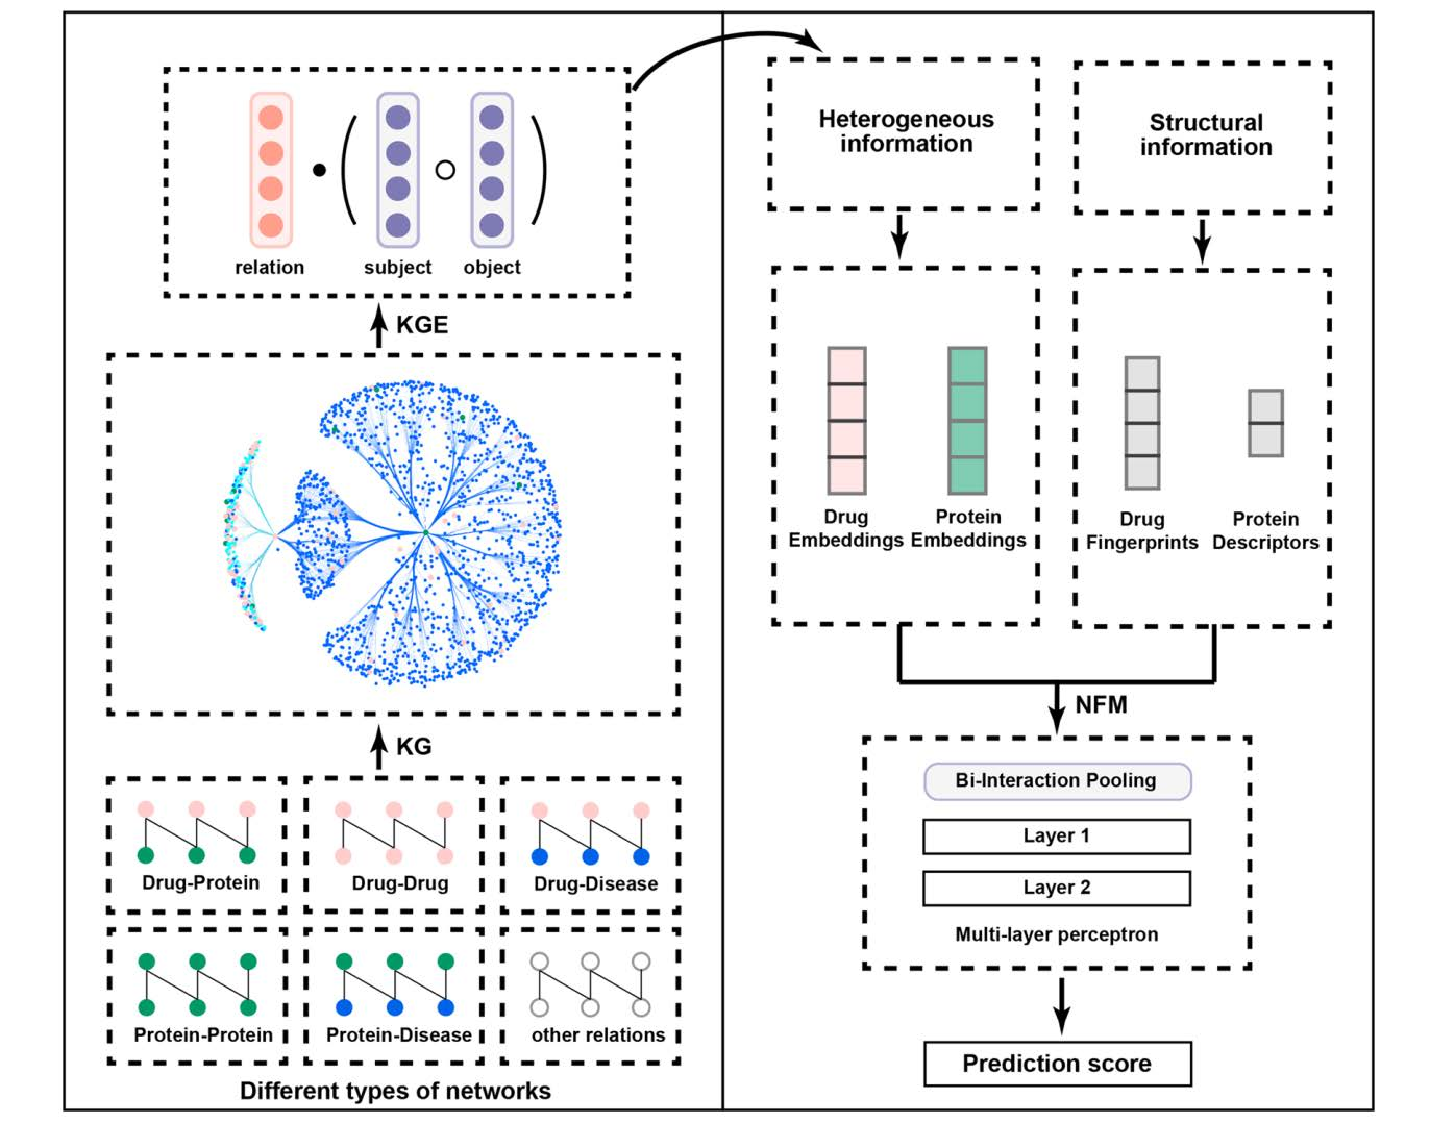
\includegraphics[
        width=0.95\textwidth,
        height=0.78\textheight,
        keepaspectratio
    ]{images/chapter5_overall_architecture.pdf}
}{
    \fbox{
        \parbox[c][5.2cm][c]{0.9\textwidth}{
            \centering
            \textbf{KGE-NFM architecture placeholder}\\[0.4cm]
            Biomedical KG $\rightarrow$ DistMult or CompGCN encoder
            $\rightarrow$ drug/protein embeddings $\rightarrow$ structural
            descriptors $\rightarrow$ NFM $\rightarrow$ DTI probability\\[0.4cm]
            Insert: \texttt{images/chapter5\_overall\_architecture.pdf}
        }
    }
}
\caption{KGE-NFM framework with alternative DistMult and CompGCN encoders}
\label{fig:kge_nfm_architecture}
\end{figure}

\section{Problem Formulation}

\subsection{DTI Prediction Objective}

For a drug $d$ and protein $p$, KGE-NFM estimates:

\begin{equation}
    \hat{y}_{dp}=F(d,p),
\end{equation}
where $\hat{y}_{dp}$ is the probability that the candidate pair interacts.
The supervised label is $y_{dp}\in\{0,1\}$.

\subsection{Two-Stage Learning Objective}

The first stage learns KG representations using an encoder
$g_{\theta}$:

\begin{equation}
    \mathbf{z}_{d}=g_{\theta}(d,\mathcal{G}),
    \qquad
    \mathbf{z}_{p}=g_{\theta}(p,\mathcal{G}),
\end{equation}
where $g_{\theta}$ is instantiated as either DistMult or CompGCN.

The second stage predicts the DTI label from KG embeddings and structural
descriptors:

\begin{equation}
    \hat{y}_{dp}
    =
    \operatorname{NFM}
    \left(
        \mathbf{z}_{d},
        \mathbf{z}_{p},
        \mathbf{s}_{d},
        \mathbf{s}_{p}
    \right).
\end{equation}

The two stages are trained sequentially for each cross-validation fold. The
KGE model is trained first, after which its drug and protein embeddings are
used as input fields for NFM.

\section{Fold-Specific Knowledge Graph Construction}

\subsection{Supporting Biomedical Triples}

Let $\mathcal{T}_{support}$ denote the biomedical triples that provide context
beyond the target DTI labels. These triples include pathway, annotation,
domain, family, interaction, and other relations available in the selected
dataset.

\subsection{Positive Training DTI Triples}

For each cross-validation fold, positive DTI triples from the training split
are added to the supporting KG:

\begin{equation}
    \mathcal{T}_{train}^{KGE}
    =
    \mathcal{T}_{support}
    \cup
    \mathcal{T}_{DTI,train}^{+}.
    \label{eq:kge_training_graph}
\end{equation}

This construction allows the encoder to learn from both the biomedical graph
and the DTI evidence available in the current training fold.

\subsection{Negative Sampling}

Negative KGE triples are generated during training by replacing the head or
tail of a positive triple. Both encoder configurations use basic negative
sampling and the margin ranking objective in
Equation~\ref{eq:background_kge_loss}. Keeping the sampling strategy fixed
reduces confounding factors in the encoder comparison.

\subsection{Inverse Relations}

The CompGCN configuration augments the graph with inverse triples. For an
original edge $(u,r,v)$, the inverse edge is $(v,r^{-1},u)$. This permits
information propagation in both directions while preserving the semantic
distinction between the original and inverse relations. DistMult uses the
original training triples without graph-convolutional neighborhood expansion.

\subsection{Prevention of Test-Label Leakage}

Only positive DTI triples from the training fold are included in
$\mathcal{T}_{train}^{KGE}$. Test DTI labels are excluded from KGE and NFM
training. Preprocessing transformations, including feature scaling and PCA,
are fitted on training data and then applied to the test fold.

\section{DistMult Encoder}

\subsection{Entity and Relation Representations}

DistMult assigns a vector to every entity and relation
\cite{yang2015embedding}. For a triple $(h,r,t)$:

\begin{equation}
    \mathbf{h},\mathbf{r},\mathbf{t}
    \in
    \mathbb{R}^{k}.
\end{equation}

Its trainable parameters are the entity embedding matrix and relation
embedding matrix. No explicit neighborhood aggregation is performed.

\subsection{DistMult Scoring Function}

DistMult scores a triple using a diagonal bilinear interaction:

\begin{equation}
    f_{\mathrm{DM}}(h,r,t)
    =
    \mathbf{h}^{\top}
    \operatorname{diag}(\mathbf{r})
    \mathbf{t}
    =
    \sum_{i=1}^{k}h_i r_i t_i.
    \label{eq:distmult_score}
\end{equation}

The diagonal form provides an efficient relation-dependent compatibility score
without requiring a full $k\times k$ matrix for every relation.

\subsection{KGE Training Objective}

The DistMult score in Equation~\ref{eq:distmult_score} is substituted into the
margin ranking loss in Equation~\ref{eq:background_kge_loss}. The model is
trained with Adam and basic negative sampling so that positive triples receive
higher scores than corrupted triples.

\subsection{Drug and Protein Embedding Extraction}

After KGE training, drug and protein representations are read from the learned
entity embedding table:

\begin{equation}
    \mathbf{z}_{d}^{DM}=\mathbf{E}[d],
    \qquad
    \mathbf{z}_{p}^{DM}=\mathbf{E}[p].
\end{equation}

These vectors form the KG fields of the DistMult-based KGE-NFM configuration.

\subsection{Advantages and Structural Limitations}

DistMult is computationally efficient, scalable, and provides compact entity
representations. However, its score is symmetric for a fixed relation:

\begin{equation}
    f_{\mathrm{DM}}(h,r,t)
    =
    f_{\mathrm{DM}}(t,r,h).
\end{equation}

It also learns through triple-level scoring without explicitly aggregating
relation-aware neighborhoods. These properties motivate evaluating CompGCN as
an alternative encoder within the same KGE-NFM framework.

\section{CompGCN Encoder}

\subsection{Graph Augmentation}

CompGCN is a multi-relational graph convolutional encoder
\cite{vashishth2020composition}. Unlike a standard GCN, it must account for
both the semantic type and direction of every edge.

The standard update in Equation~\ref{eq:background_gcn_update} uses one shared
transformation and does not distinguish relation semantics. The relational
update in Equation~\ref{eq:background_relational_gcn_update} introduces
$\mathbf{W}_{r}^{k}$ for each relation, but its parameter count grows with the
number of relation types. CompGCN retains relational message passing while
replacing relation-specific matrices with entity--relation composition and
three direction-specific transformations.

For each original triple:

\begin{equation}
    (u,r,v),
\end{equation}

the graph is augmented with an inverse triple:

\begin{equation}
    (v,r^{-1},u),
\end{equation}

and a self-loop relation is associated with each entity. The resulting
relation set contains original relations, inverse relations, and a self-loop
relation. Original edges preserve the observed direction, inverse edges permit
information to propagate in the reverse direction, and self-loops retain the
entity's own representation during aggregation. In the implementation,
inverse triples are created when the CompGCN triples factory is constructed.

At layer $k$, CompGCN maintains an entity representation
$\mathbf{h}_{v}^{k}$ for every entity $v$ and a relation representation
$\mathbf{h}_{r}^{k}$ for every relation $r$. Thus, relations are learned
components of the encoder rather than fixed edge labels.

\subsection{Entity--Relation Composition}

Before aggregation, a neighboring entity representation is composed with the
relation embedding:

\begin{equation}
    \mathbf{m}_{u,r}^{k}
    =
    \phi
    \left(
        \mathbf{h}_{u}^{k},
        \mathbf{h}_{r}^{k}
    \right).
\end{equation}

The implementation supports subtraction, element-wise multiplication, and
circular correlation. These operators correspond to different assumptions
about how a relation modifies an entity representation:

\begin{align}
    \phi_{sub}(\mathbf{h}_{u},\mathbf{h}_{r})
    &=
    \mathbf{h}_{u}-\mathbf{h}_{r}, \\
    \phi_{mult}(\mathbf{h}_{u},\mathbf{h}_{r})
    &=
    \mathbf{h}_{u}\odot\mathbf{h}_{r}, \\
    \phi_{corr}(\mathbf{h}_{u},\mathbf{h}_{r})
    &=
    \mathbf{h}_{u}\star\mathbf{h}_{r},
\end{align}
where $\odot$ denotes element-wise multiplication and $\star$ denotes circular
correlation. Subtraction follows a translation-style interpretation,
multiplication applies relation-dependent feature gating, and circular
correlation captures interactions across embedding dimensions. The main
configuration uses multiplication:

\begin{equation}
    \phi
    \left(
        \mathbf{h}_{u}^{k},
        \mathbf{h}_{r}^{k}
    \right)
    =
    \mathbf{h}_{u}^{k}\odot\mathbf{h}_{r}^{k}.
\end{equation}

Consequently, the same neighboring entity can send different messages through
different relations. This is the central distinction between CompGCN and a
relation-agnostic graph convolution.

\subsection{Node Representation Update}

The representation of node $v$ is updated by aggregating composed messages:

\begin{equation}
    \mathbf{h}_{v}^{k+1}
    =
    \sigma
    \left(
        \sum_{(u,r)\in\mathcal{N}(v)}
        \mathbf{W}_{\lambda(r)}^{k}
        \phi
        \left(
            \mathbf{h}_{u}^{k},
            \mathbf{h}_{r}^{k}
        \right)
    \right),
    \label{eq:compgcn_node_update}
\end{equation}
where $\mathcal{N}(v)$ is the relational neighborhood of $v$,
$\mathbf{W}_{\lambda(r)}^{k}$ is selected according to edge direction, and
$\sigma$ is a nonlinear activation. The direction function is defined as:

\begin{equation}
    \lambda(r)
    \in
    \{O,I,S\},
\end{equation}
where $O$, $I$, and $S$ indicate original, inverse, and self-loop edges,
respectively. The corresponding transformations are
$\mathbf{W}_{O}^{k}$, $\mathbf{W}_{I}^{k}$, and $\mathbf{W}_{S}^{k}$.
CompGCN therefore does not require a separate full transformation matrix for
every relation. Relation-specific semantics are carried by
$\mathbf{h}_{r}^{k}$ and the composition function, while the transformation
matrices are shared according to edge direction. This design limits parameter
growth when the graph contains many relation types.

Stacking $L$ CompGCN layers repeats this update using the representations from
the preceding layer. The final entity representation
$\mathbf{h}_{v}^{L}$ therefore incorporates relation-conditioned information
from an $L$-hop neighborhood, subject to the graph connectivity and learned
transformations.

\subsection{Relation Representation Update}

Relation embeddings are updated at each CompGCN layer:

\begin{equation}
    \mathbf{h}_{r}^{k+1}
    =
    \mathbf{W}_{rel}^{k}
    \mathbf{h}_{r}^{k}.
    \label{eq:compgcn_relation_update}
\end{equation}

This update keeps relation representations aligned with the evolving entity
embedding space. Entity and relation states therefore evolve together across
the encoder. The trainable parameters include the initial entity and relation
representations, the direction-specific matrices at each layer, and the
relation transformation matrices. During training, gradients from the
link-prediction loss update $\mathbf{W}_{O}^{k}$, $\mathbf{W}_{I}^{k}$,
$\mathbf{W}_{S}^{k}$, $\mathbf{W}_{rel}^{k}$, and the initial entity and
relation embeddings jointly.

The original CompGCN formulation also proposes basis decomposition for graphs
with many relations. A relation embedding can be represented as:

\begin{equation}
    \mathbf{h}_{r}^{0}
    =
    \sum_{b=1}^{B}
    \alpha_{br}\mathbf{v}_{b},
\end{equation}
where $\mathbf{v}_{b}$ is a learned basis vector and $\alpha_{br}$ is the
coefficient of basis $b$ for relation $r$. This reduces relation-embedding
parameters. Basis decomposition is part of the general CompGCN method; the
project configuration primarily controls embedding dimension, layer count,
dropout, and composition operator through PyKEEN.

% Replace document/images/chapter5_compgcn_message_passing.pdf with the final
% CompGCN neighborhood aggregation diagram.
\begin{figure}[H]
\centering
\IfFileExists{images/chapter5_compgcn_message_passing.pdf}{
    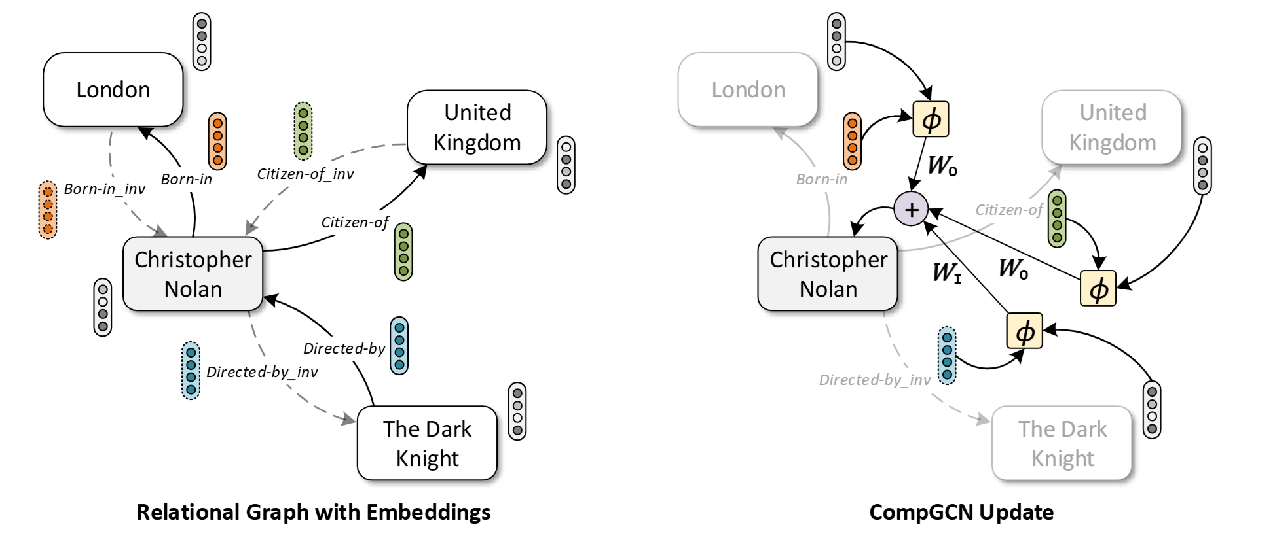
\includegraphics[width=0.9\textwidth]{images/chapter5_compgcn_message_passing.pdf}
}{
    \fbox{
        \parbox[c][5.2cm][c]{0.86\textwidth}{
            \centering
            \textbf{CompGCN message-passing diagram placeholder}\\[0.4cm]
            Show original, inverse, and self-loop messages transformed through
            $\mathbf{W}_{\lambda(r)}\phi(\mathbf{h}_u,\mathbf{h}_r)$.\\[0.4cm]
            Insert: \texttt{images/chapter5\_compgcn\_message\_passing.pdf}
        }
    }
}
\caption{Relation-aware message passing in the CompGCN encoder}
\label{fig:compgcn_message_passing}
\end{figure}

\subsection{Link-Prediction Decoder}

CompGCN acts as an encoder that produces enriched entity and relation
representations. These representations are passed to a KGE decoder that assigns
a plausibility score to each triple:

\begin{equation}
    f_{CG}(h,r,t)
    =
    \operatorname{Dec}
    \left(
        \mathbf{h}_{h}^{L},
        \mathbf{h}_{r}^{L},
        \mathbf{h}_{t}^{L}
    \right).
\end{equation}

The CompGCN paper treats the encoder and decoder as separate components and
evaluates the encoder with TransE, DistMult, and ConvE scoring functions. This
separation is important: CompGCN determines how entity and relation
representations are enriched through graph convolution, whereas the decoder
determines how the resulting representations are scored for link prediction.

In this project, the PyKEEN CompGCN model supplies the link-prediction score
used during KGE training. The full encoder--decoder model is optimized with the
same margin ranking loss, Adam optimizer, and basic negative-sampling strategy
used for the DistMult configuration. Holding the training objective constant
allows the experiment to focus on the effect of relation-aware representation
learning.

\subsection{Drug and Protein Embedding Extraction}

After the final CompGCN layer, enriched drug and protein embeddings are
extracted:

\begin{equation}
    \mathbf{z}_{d}^{CG}=\mathbf{h}_{d}^{L},
    \qquad
    \mathbf{z}_{p}^{CG}=\mathbf{h}_{p}^{L}.
\end{equation}

These embeddings form the KG fields of the CompGCN-based KGE-NFM
configuration. The downstream feature construction and NFM predictor remain
the same as in the DistMult configuration. Thus, CompGCN is used as a
representation encoder inside KGE-NFM rather than as the final DTI classifier.

\section{Drug--Target Feature Construction}

\subsection{Drug and Protein KG Embeddings}

For either encoder, the candidate pair contains separate drug and protein KG
fields, $\mathbf{z}_{d}$ and $\mathbf{z}_{p}$. Keeping them separate allows
NFM to learn interactions between the two entity representations instead of
merging them before prediction.

\subsection{Morgan Fingerprints}

Each drug is represented by a Morgan fingerprint
$\mathbf{s}_{d}\in\mathbb{R}^{1024}$. The binary fingerprint encodes local
molecular substructures and supplies intrinsic chemical information that is
not directly represented by the KG embedding.

\subsection{Protein CTD Descriptors}

Each target protein is represented by a CTD descriptor
$\mathbf{s}_{p}\in\mathbb{R}^{147}$. CTD features summarize the composition,
transition, and distribution of amino acid property groups.

\subsection{Feature Scaling and Optional PCA}

All feature fields are scaled using parameters fitted on the training fold.
PCA can optionally reduce the drug and protein KG embeddings. PCA is fitted
separately on the training embeddings and applied unchanged to the test
embeddings, preventing test-data leakage.

\subsection{Final Pair Representation}

The four default KGE-NFM fields are:

\begin{equation}
    \mathcal{F}_{dp}
    =
    \left\{
        \mathbf{z}_{d},
        \mathbf{z}_{p},
        \mathbf{s}_{d},
        \mathbf{s}_{p}
    \right\}.
    \label{eq:kge_nfm_fields}
\end{equation}

Conceptually, their concatenated representation is:

\begin{equation}
    \mathbf{x}_{dp}
    =
    [
        \mathbf{z}_{d}
        \mathbin{\Vert}
        \mathbf{z}_{p}
        \mathbin{\Vert}
        \mathbf{s}_{d}
        \mathbin{\Vert}
        \mathbf{s}_{p}
    ],
\end{equation}
although the implemented NFM processes these inputs as separate feature fields.

\section{Neural Factorization Machine}

\subsection{Feature-Field Projection}

The project uses a field-based NFM implementation derived from the NFM
principle in \cite{he2017neural}. Each input field
$\mathbf{x}_{dp}^{(m)}\in\mathbb{R}^{D_m}$ is projected into a shared latent
dimension:

\begin{equation}
    \mathbf{u}_{m}
    =
    \mathbf{P}_{m}\mathbf{x}_{dp}^{(m)}+\mathbf{b}_{m}.
    \label{eq:nfm_field_projection}
\end{equation}

This projection makes KG embeddings, fingerprints, and CTD descriptors
compatible for field-level interaction modeling.

\subsection{Bi-Interaction Pooling}

The projected fields are combined using Bi-Interaction pooling:

\begin{equation}
    \mathbf{f}_{BI}
    =
    \frac{1}{2}
    \left[
        \left(
            \sum_{m=1}^{M}\mathbf{u}_{m}
        \right)^2
        -
        \sum_{m=1}^{M}\mathbf{u}_{m}^{2}
    \right].
    \label{eq:nfm_bi_interaction}
\end{equation}

This operation summarizes pairwise interactions among drug KG, protein KG,
drug structure, and protein descriptor fields.

\subsection{Hidden Layers}

The interaction vector is processed by fully connected hidden layers:

\begin{equation}
    \mathbf{a}^{(l+1)}
    =
    \operatorname{ReLU}
    \left(
        \mathbf{W}^{(l)}\mathbf{a}^{(l)}+\mathbf{b}^{(l)}
    \right),
\end{equation}
where $\mathbf{a}^{(0)}=\mathbf{f}_{BI}$. Dropout can be applied after hidden
activations as regularization.

\subsection{DTI Prediction Function}

The final logit combines field-level linear terms and the nonlinear interaction
network:

\begin{equation}
    o_{dp}
    =
    \sum_{m=1}^{M}
    \left(
        \mathbf{a}_{m}^{\top}\mathbf{x}_{dp}^{(m)}+c_m
    \right)
    +
    \operatorname{MLP}(\mathbf{f}_{BI}).
\end{equation}

The predicted DTI probability is:

\begin{equation}
    \hat{y}_{dp}=\operatorname{sigmoid}(o_{dp}).
\end{equation}

\subsection{Binary Classification Objective}

NFM is optimized using binary cross-entropy:

\begin{equation}
    \mathcal{L}_{DTI}
    =
    -\frac{1}{N}
    \sum_{i=1}^{N}
    \left[
        y_i\log(\hat{y}_i)
        +(1-y_i)\log(1-\hat{y}_i)
    \right].
\end{equation}
